
\documentclass{beamer}

\mode<presentation>{\usetheme{Madrid}}

\usepackage[utf8]{inputenc}
\usepackage[ngerman]{babel}
\usepackage{amsmath, amssymb, amsthm}
\usepackage{graphicx}
\usepackage{booktabs}
\usepackage{tikz}

\usepackage{subcaption}


\author[Philipp Geier]{}
\title[Sorting Colored Balls in Colored Tubes]{Sorting Colored Balls in Colored Tubes \\ von Ernst Althaus et. al}
\institute[Universität Trier]{}
\date{}
\beamertemplatenavigationsymbolsempty

\usepackage{enumitem}
\newlist{arrowlist}{itemize}{1}
\setlist[arrowlist]{label=$\Rightarrow$}
\newlist{pointlist}{itemize}{1}
\setlist[pointlist]{label=$\circ$}
\newlist{enumlist}{enumerate}{1}
\setlist[enumlist]{label=\arabic*.}

%—-------------------------------------------------------------

\begin{document}
{
  \usebackgroundtemplate{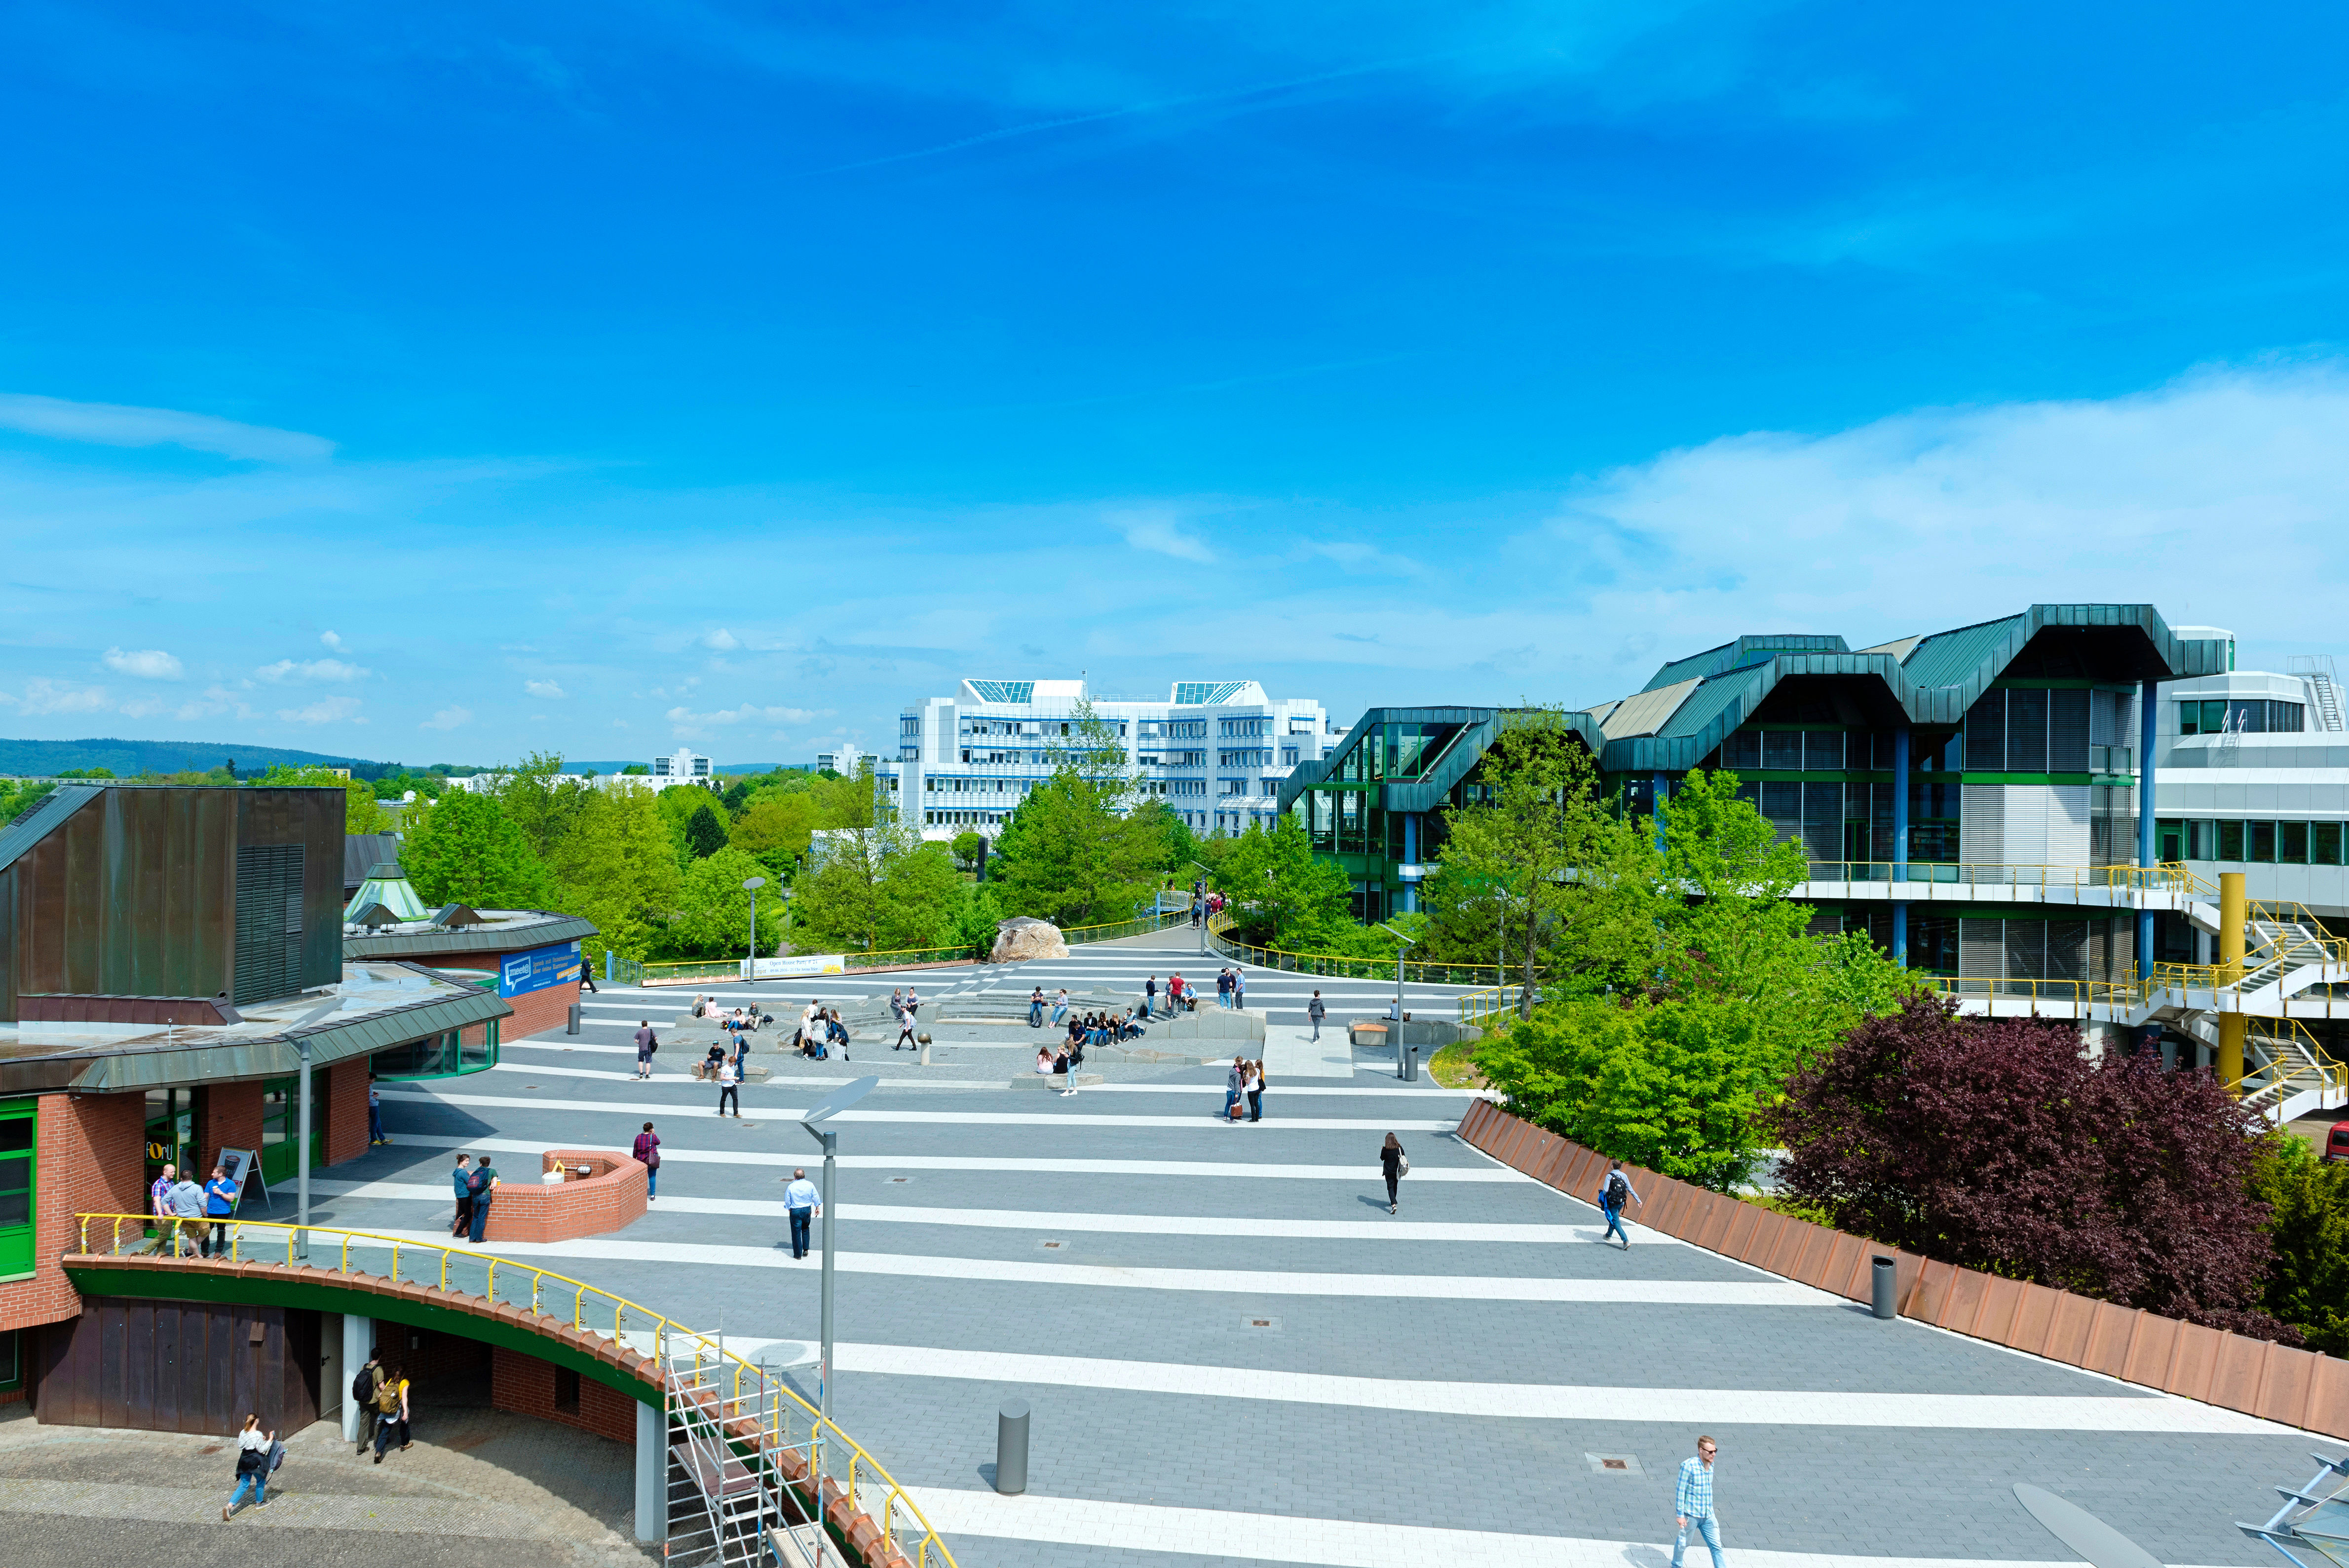
\includegraphics[width=1.2\paperwidth]{unitrier}}
  \begin{frame}
    \maketitle
  \end{frame}
}
    
    %\begin{frame}
       % \frametitle{Inhalt}
		%\tableofcontents
	%\end{frame}
	
%—------------------------------------------------------


\begin{frame}{Ziel: Kleinste Anzahl an Zügen}
	\begin{figure}[ht]
		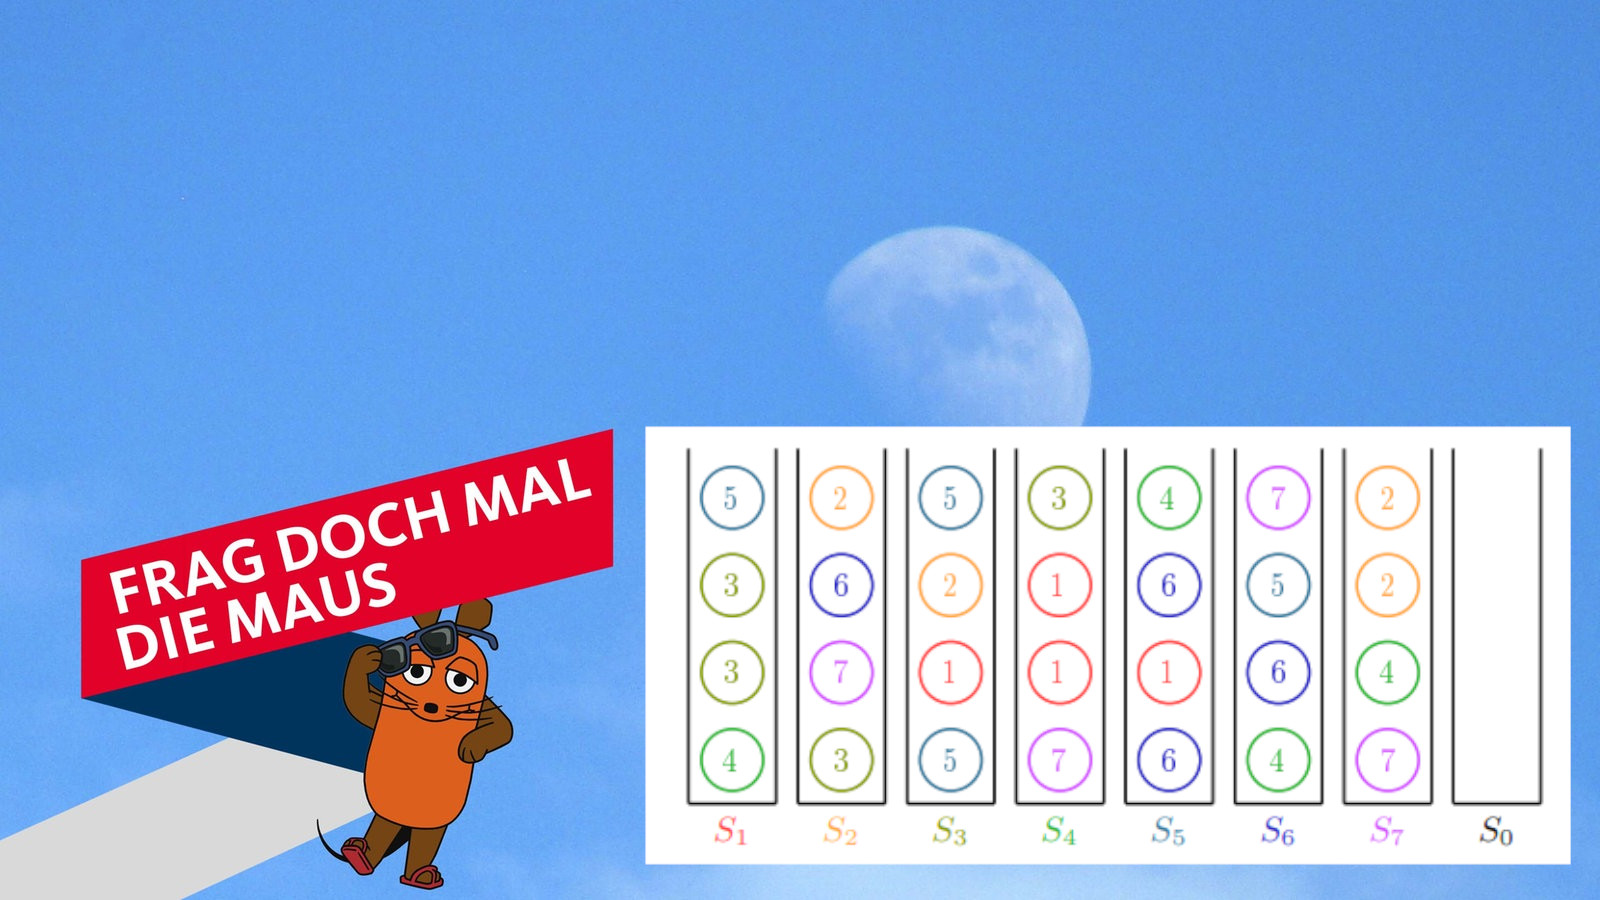
\includegraphics[width=\textwidth]{maus}
    \end{figure}
\end{frame}

\begin{frame}{Idee}
	\begin{pointlist}
		\item Feedback Arc Set Problem (FAS) ist ähnlich zum Spiel mit unbegrenzter Höhe
		\item Konstruktion des Spiels (SCBT) als Graphen 
		\item Reduktion des Problems auf FAS
		\item FAS ist NP-vollständig, somit auch SCBT
	\end{pointlist}
\end{frame}

\begin{frame}{Definitionen}
	\begin{pointlist}
		\item Menge an Farben $C=\{1,\dots c\}$ mit festem $c\in \mathbb{N}$
		\item $c+1$ Tuben der Höhe $h_i\in\mathbb{N}$ in den Farben und eine farblos
		\item Bis zu $h_i$ Bälle pro Farbe
		\item Konfiguration $S$ einer Tube ist eine Sequenz $(b_1,\dots,b_l)$ mit $l\leq h$
		\item Tube-Rack $(T_0, T_1,\dots,T_c)$ hat Höhenprofil $H=(h_0,\dots,h_c)$ und Ersatztube $T_0$
		\end{pointlist}
		\end{frame}
\begin{frame}{Definitionen}
	\begin{pointlist}
		\item Konfiguration eines Tube-Racks ist $S=(S_0,\dots,S_c)$ mit $|S_i| \leq h_i$
		\item Zug $(i,j)$ heißt valide, falls $|S_i|\geq 1$ und $|S_j| < h_j$
		\item Finale Konfiguration ist $S=(S_0,\dots, S_0)$ mit $S_0 = ()$ und $S_i =(i,\dots,i)$ für $1\leq i \leq c$
		\item $i$-farbiger Ball ist in finaler Position, falls er in Tube $i$ ist und alle Bälle darunter Farbe $i$ haben
	\end{pointlist}
\end{frame}

\begin{frame}{Probleme}
	\begin{pointlist}
		\item SCBT-Problem:
		\begin{arrowlist}
 			\item Instanz $(H,S,k)$ mit $k$ validen Zügen
		\end{arrowlist}
		\item Restricted SCBT-Problem (RSCBT):
		\begin{arrowlist}
 			\item Anzahl Bälle der Farbe $i$ gleich der Höhe $h\in\mathbb{N}$ mit dem Höhenprofil $H=(h,\dots,h)$
		\end{arrowlist}
	\end{pointlist}
\end{frame}

\begin{frame}{Lemma 1}
\begin{enumlist}
\item Falls die Anzahl der Bälle der Farbe $i$ $h$ entspricht für alle $1 \leq i \leq c$, hat $((h,\dots,h),S,c\cdot h\cdot (2h+1))$ eine Lösung, 
\item Falls $(H,S,k)$ eine Lösung hat und $H' \geq H$ gilt, dann hat $(H',S,k)$ auch eine Lösung
\item Falls $(H,S,k)$ mit $H=(\infty,\dots, \infty)$ eine Lösung hat, dann existiert eine Lösung mit: \begin{pointlist}
\item Bälle in finaler Position werden nicht bewegt
\item Jeder andere wird 1- oder 2-mal bewegt
\end{pointlist}
\item Falls $((\infty, \dots,\infty),S,k)$ eine Lösung hat und $H=(\infty, h_1,\dots, h_c)$ mit $h_i \geq \max(|s_i|,b_i)$ gilt, dann hat $(H,S,k)$ eine Lösung
\end{enumlist}
\end{frame}

\begin{frame}{Feedback Arc Set (FAS)}
\begin{pointlist}
\item geg.: gerichteter Multigraph G=(V,E) und $k\in\mathbb{N}_0$
\item ges.: $\exists E' \subseteq E$ mit $|E'|\leq k$, sodass $G'(V,E\backslash E')$ azyklisch ist
\end{pointlist}
\vspace*{1cm}
\begin{arrowlist}
\item Nach Karp (1972) NP-vollständig
\end{arrowlist}
\end{frame}

\begin{frame}{Konstruktion}
\begin{pointlist}
\item $V=\{1,\dots,n\}$ und $G$ azyklischqazre  
\end{pointlist}
\end{frame}

\begin{frame}{Lemma 2}
\end{frame}

\begin{frame}{Beweis (Hinrichtung)}
\end{frame}

\begin{frame}{Beweis (Rückrichtung)}
\end{frame}

\begin{frame}{Beweis (Rückrichtung)}
\end{frame}

\begin{frame}{Definition DFVS}
\end{frame}

\begin{frame}{Lower Bounds}
\end{frame}

\begin{frame}{Algorithmus}
\end{frame}

\begin{frame}{Related Work}
	\begin{pointlist}
		\item Sortieren von farbigen Bällen in farblosen Tuben. Bälle nur auf Bälle gleicher Farbe oder in leere Tuben (Reduktion von 3-Partition)
		\item $k$ $i$-farbige Bälle in umgekehrter Reihenfolge. Nur adjazente Bälle können getauscht werden 
		\item Reales Problem: Container in Terminalen, um Effizienz im Lagerplatz zu steigern, unproduktive Züge beim Stapeln zu vermeiden und sich an Planungseinschränkungen zu halten 
	\end{pointlist}
\end{frame}



\begin{frame}{}
  \centering \Huge
  \emph{Fin}
\end{frame}


	
    	
    	
    	
\end{document}
